\section{Feed-forward neural networks}\label{sec:super}

Before introducing the vanilla feed-forward neural nets, let us set up necessary notations for the rest of this section. We focus primarily on classification problems, as regression problems can be addressed similarly. Given the training dataset $\{ (y_i, \xx_i )\}_{1\leq i\leq n}$ where $y_i \in [K] \triangleq \{1,2,\ldots,K\}$ and $\xx_{i} \in \R^d$ are independent across $i \in [n]$, supervised learning aims at finding a (possibly random) function $\hat f(\xx)$ that predicts the outcome $y$ for a new input $\xx$, assuming $(y, \xx)$ follows the same distribution as $(y_i, \xx_i )$. In the terminology of machine learning, the input $\xx_i$ is often called the \textit{feature}, the output $y_i$ called the \textit{label}, and the pair $(y_i,\bm{x}_i)$ is an \textit{example}. The function $\hat f$ is called the \textit{classifier}, and estimation of $\hat f$ is \textit{training} or \textit{learning}. The performance of $\hat f$ is evaluated through the prediction error $\P(y \neq \hat f(\xx))$, which can be often estimated from a separate test dataset.

As with classical statistical estimation, for each $k \in [K]$, a classifier approximates the conditional probability $\P(y = k | \xx)$ using a function $f_k(\xx; \btheta_k)$ parametrized by $\btheta_k$. Then the category with the highest probability is predicted. Thus, learning is essentially estimating the parameters $\btheta_k$. In statistics, one of the most popular methods is (multinomial) logistic regression, which stipulates a specific form for the functions $f_k(\xx; \btheta_k)$: let $z_k = \xx^\top \bbeta_k + \alpha_k$ and $f_k(\xx; \btheta_k) = Z^{-1} \exp(z_k)$ where $Z = \sum_{k=1}^K \exp(z_k)$ is a normalization factor to make $\{f_k(\xx; \btheta_k)\}_{1\leq k \leq K}$ a valid probability distribution. It is clear that logistic regression induces linear decision boundaries in $\mathbb{R}^{d}$, and hence it is restrictive in modeling nonlinear dependency between $y$ and $\xx$. The deep neural networks we introduce below provide a flexible framework for modeling nonlinearity in a fairly general way.

\subsection{Model setup}

From the high level, deep neural networks (DNNs) use composition of a series of simple nonlinear functions to model nonlinearity
\begin{equation*}
\hh^{(L)} = \bg^{(L)} \circ  \bg^{(L-1)} \circ \ldots \circ \bg^{(1)} (\xx),
\end{equation*}
where $\circ$ denotes composition of two functions and $L$ is the number of hidden layers, and is usually called \emph{depth} of a NN model. Letting $\bm{h}^{(0)}\triangleq\bm{x}$, one can recursively define
$\hh^{(l)} =  \bg^{(l)} \big(\bm{h}^{(l-1)}\big)$ for all $\ell = 1,2,\ldots, L$. The \textit{feed-forward neural networks}, also called the \textit{multilayer perceptrons} (MLPs), are neural nets with a specific choice of $\bg^{(l)}$: for $\ell = 1,\ldots,L$, define
\begin{equation}\label{eq:fc}
\hh^{(\ell)} = \bg^{(l)} \big(\bm{h}^{(l-1)}\big) \triangleq \bsigma \big(\bW^{(\ell)} \hh^{(\ell-1)} + \bb^{(\ell)}  \big),
\end{equation}
where $\bW^{(l)}$ and  $\bb^{(l)}$ are the weight matrix and the bias$\,$/$\,$intercept, respectively, associated with the $l$-th layer, and $\bsigma(\cdot)$ is usually a simple given (known) nonlinear function called the \textit{activation function}. In words, in each layer $\ell$, the input vector $\hh^{(\ell-1)}$ goes through an affine transformation first and then passes through a fixed nonlinear function $\bsigma(\cdot)$. See Figure~\ref{fig:FFNN} for an illustration of a simple MLP with two hidden layers. The activation function $\bsigma(\cdot)$ is usually applied element-wise, and a popular choice is the ReLU (Rectified Linear Unit) function:
\begin{equation}
[\bsigma(\zz)]_j = \max\{ z_j, 0 \}.
\end{equation}
Other choices of activation functions include leaky ReLU, $\tanh$ function \citep{maas2013rectifier} and the classical sigmoid function $(1+e^{-z})^{-1}$, which is less used now.

%It is worthwhile noting that the ReLU activation function is a crucial element in most deep learning models. Its popularity is largely due to the fact that its derivative is either $0$ or $1$, which makes training more efficient. See Section~\ref{sec:opt} for discussion on numerical stability. %\TODO{add a figure?}

\begin{figure}
\centering
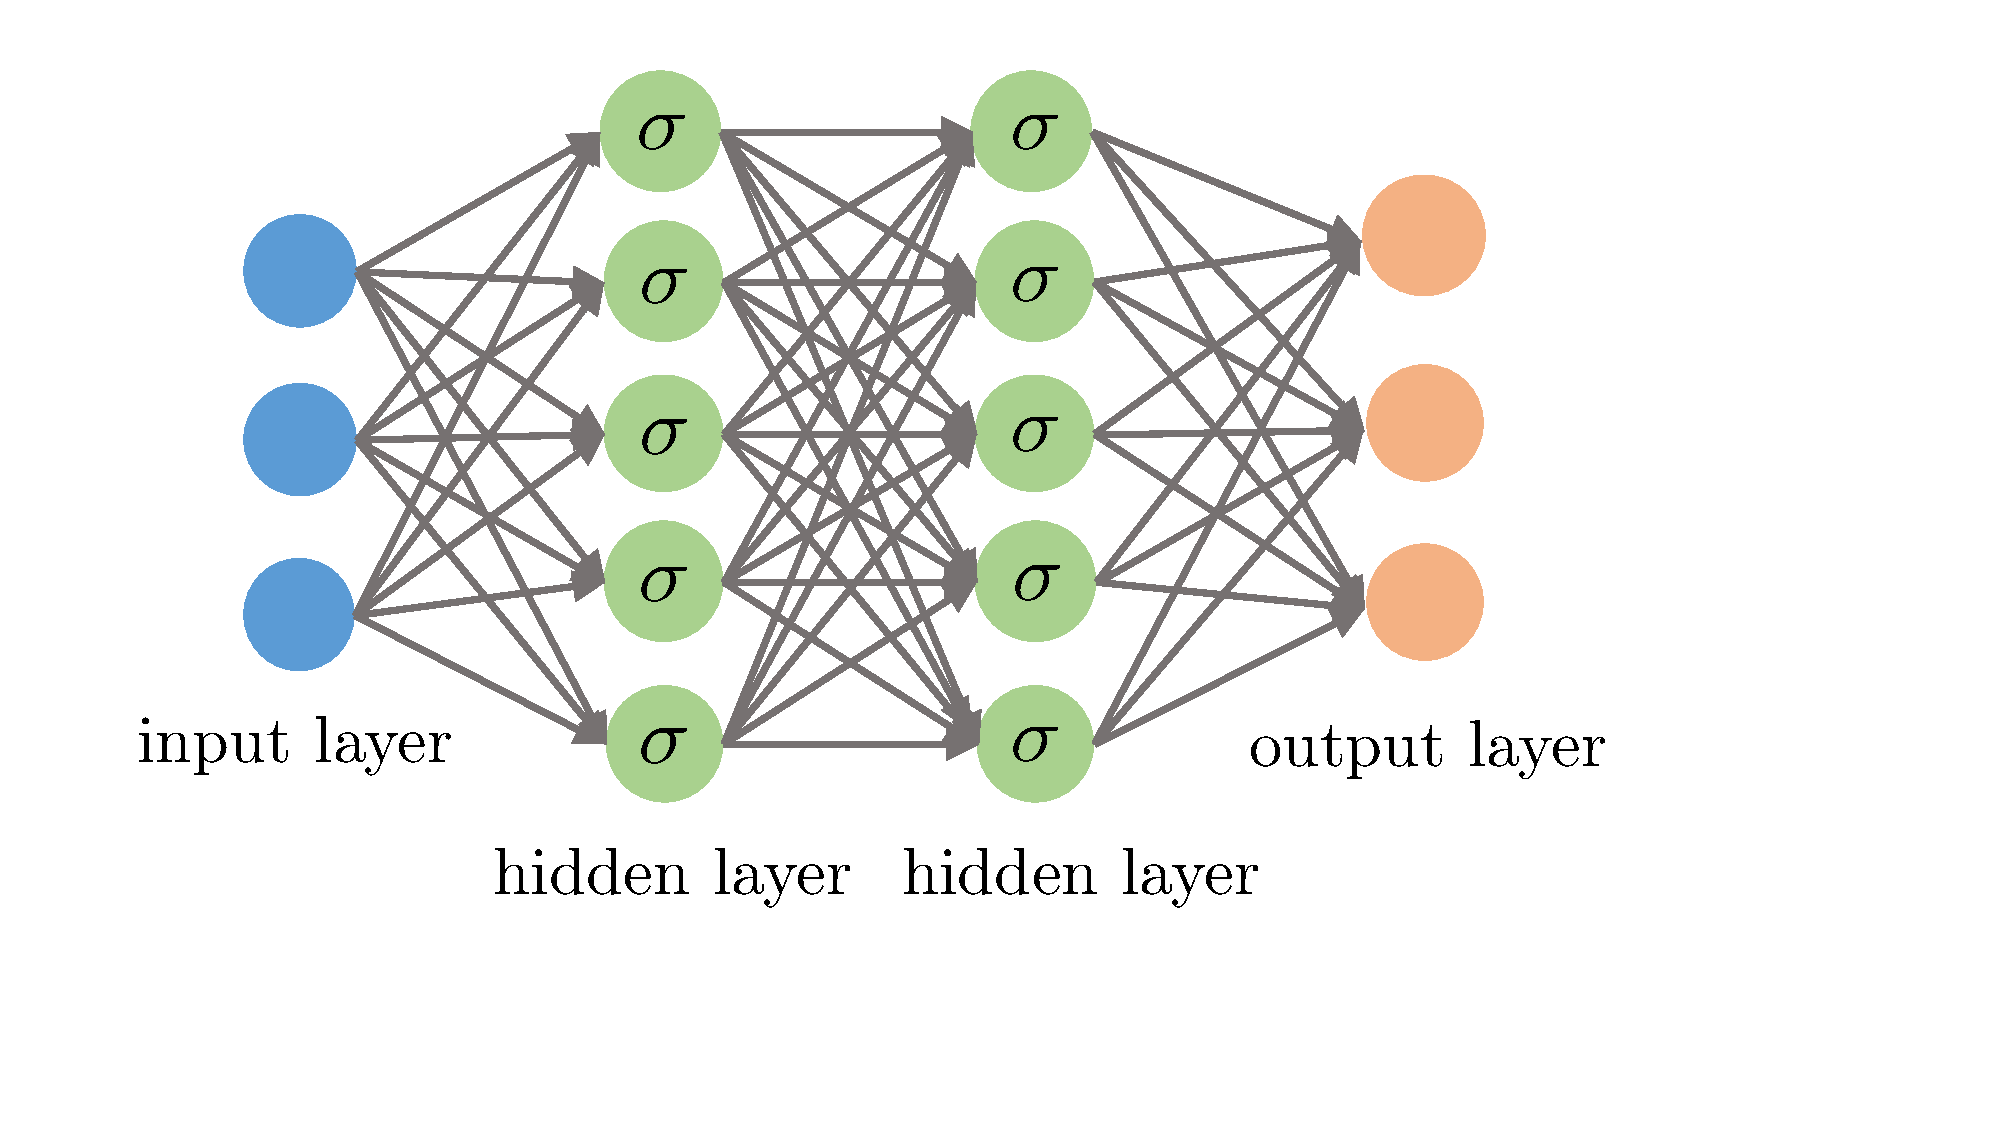
\includegraphics[scale=0.4]{MLP}\caption{A feed-forward neural network with an input layer, two hidden layers and an output layer. The input layer represents raw features $\{\bm{x}_{i}\}_{1\leq i\leq n}$. Both hidden layers compute an affine transform (a.k.s. indices) of the input and then apply an element-wise activation function $\bsigma(\cdot)$. Finally, the output returns a linear transform followed by the softmax activation (resp.~simply a linear transform) of the hidden layers for the classification (resp.~regression) problem. \label{fig:FFNN}}
\end{figure}

Given an output $\hh^{(L)}$ from the final hidden layer and a label $y$, we can define a loss function to minimize. A common loss function for classification problems is the multinomial logistic loss. Using the terminology of deep learning, we say that $\hh^{(L)}$ goes through an affine transformation and then the \textit{soft-max} function:
\begin{equation*}
f_k(\xx; \btheta) \triangleq  \frac{\exp(z_k)}{\sum_k \exp(z_k)}, \quad \forall\, k\in[K], \qquad \where~ \zz = \bW^{(L+1)} \hh^{(L)} + \bb^{(L+1)} \in \mathbb{R}^{K}.
\end{equation*}
Then the loss is defined to be the cross-entropy between the label $y$ (in the form of an indicator vector) and the score vector $ (f_1(\xx; \btheta),\ldots,f_K(\xx; \btheta))^\top$, which is exactly the negative log-likelihood of the multinomial logistic regression model:
\begin{equation}\label{eq:crossentropy}
\mathcal{L}(\ff(\xx; \btheta), y)=-\sum_{k=1}^K \bbone\{y = k\} \log p_k,
\end{equation}
where $\btheta \triangleq \{ \bW^{(\ell)}, \bb^{(\ell)}: 1\leq \ell \leq L+1\}$.
As a final remark, the number of parameters scales with both the depth $L$ and the width (i.e., the dimensionality of $\bW^{(\ell)}$), and hence it can be quite large for deep neural nets. %Here we abuse the notation $\mathcal{L}$ to denote either the loss on a single example $(y_i, \bm{x}_i)$ or the loss over the whole data $\{(y_i, \bm{x}_i)\}_{1\leq i \leq n}$. \TODO{We may use $\ell(\btheta)$ to represent the sample average.} \cm{Yes, I have adopted this in training section.}

\subsection{Back-propagation in computational graphs}
%Training neural nets is essentially the process of finding parameters to minimize the empirical loss over the whole dataset, i.e.,
%\begin{equation}\label{eq:loss-nn}
%\ell_n(\btheta) \triangleq \frac{1}{n}\sum_{i=1}^{n}\mathcal{L}(\ff(\xx_i; \btheta), y_i).
%\end{equation}

Training neural networks follows the \emph{empirical risk minimization} paradigm that minimizes the loss (e.g., (\ref{eq:crossentropy})) over all the training data. This minimization is usually done via \textit{stochastic gradient descent} (SGD). In a way similar to gradient descent, SGD starts from a certain initial value $\btheta^{0}$ and then iteratively updates the parameters $\btheta^{t}$ by moving it in the direction of the negative gradient.
%In a way similar to the gradient descent method, starting from some initial values, the parameters $\btheta^{t}$ are iteratively updated by moving a step in the direction of the negative gradient $-\nabla \ell_n(\btheta^{t})$ for certain empirical loss function $\ell_n$.
The difference is that, in each update, a small subsample $\mathcal{B} \subset [n]$ called a \textit{mini-batch}---which is typically of size 32--512---is randomly drawn and the gradient calculation is only on $\mathcal{B}$ instead of the full batch $[n]$.  This saves considerably the computational cost in calculation of gradient.  By the law of large numbers, this stochastic gradient should be close to the full sample one, albeit with some random fluctuations.  A pass of the whole training set is called an \textit{epoch}. Usually, after several or tens of epochs, the error on a validation set levels off and training is complete. See Section~\ref{sec:opt} for more details and variants on training algorithms.

The key to the above training procedure, namely SGD, is the calculation of the gradient $\nabla \ell_{\cB}(\btheta)$, where
\begin{equation}\label{eq:loss-nn}
\ell_{\cB}(\btheta) \triangleq |\cB|^{-1} \sum_{i \in \cB} \mathcal{L}(\ff(\xx_i ; \btheta), y_i).
\end{equation}
Gradient computation, however, is in general nontrivial for complex models, and it is susceptible to numerical instability for a model with large depth. Here, we introduce an efficient approach, namely \textit{back-propagation}, for computing gradients in neural networks.

%It essentially follows the principle of the gradient descent method, which is the algorithmic routine of many statistics and machine learning problems.
%This makes gradient calculation very efficient.
%For neural networks, gradient calculation is based on \textit{back-propagation} \citep{rumelhart1985learning}, which
Back-propagation \citep{rumelhart1985learning} is a direct application of the chain rule in networks. As the name suggests, the calculation is performed in a backward fashion: one first computes $\partial \ell_{\cB}/\partial \hh^{(L)}$, then $\partial \ell_{\cB}/\partial \hh^{(L-1)}$, $\ldots$, and finally $\partial \ell_{\cB}/\partial \hh^{(1)}$. For example, in the case of the ReLU activation function\footnote{The issue of non-differentiability at the origin is often ignored in implementation.}, we have the following recursive$\,$/$\,$backward relation
\begin{equation}\label{eq:grad}
\frac{\partial \ell_{\cB}}{\partial \hh^{(\ell-1)}} =  \frac{\partial \hh^{(\ell)}}{\partial \hh^{(\ell-1)}} \cdot \frac{\partial \ell_{\cB}}{\partial \hh^{(\ell)}} = (\bW^{(\ell)})^\top \mathsf{diag}\left( \bbone\{\bW^{(\ell)} \hh^{(\ell-1)} + \bb^{(\ell)}  \ge \bm{0}\}  \right) \frac{\partial \ell_{\cB}}{\partial \hh^{(\ell)}}
\end{equation}
where $\mathsf{diag}(\cdot)$ denotes a diagonal matrix with elements given by the argument. Note that the calculation of $\partial \ell_{\cB} / \partial \hh^{(\ell-1)}$ depends on $\partial \ell_{\cB} / \partial \hh^{(\ell)}$, which is the partial derivatives from the next layer. In this way, the derivatives are ``back-propagated'' from the last layer to the first layer. These derivatives $\{\partial \ell_{\cB} / \partial \hh^{(\ell)}\}$ are then used to update the parameters. For instance, the gradient update for $\bW^{(\ell)}$ is given by
\begin{equation}\label{eq:Wupdate}
\bW^{(\ell)} \leftarrow \bW^{(\ell)} - \eta \frac{\partial \ell_{\cB}}{\partial \bW^{(\ell)}}, \quad \where\quad \frac{\partial \ell_{\cB}}{\partial W_{jm}^{(\ell)}} = \frac{\partial \ell_{\cB}}{\partial h_j^{(\ell)}} \cdot \sigma' \cdot h_m^{(\ell-1)},
\end{equation}
where $\sigma' = 1$ if the $j$-th element of $\bW^{(\ell)} \hh^{(\ell-1)} + \bb^{(\ell)}$ is nonnegative, and $\sigma' = 0$ otherwise. The step size $\eta >0$, also called the \textit{learning rate}, controls how much parameters are changed in a single update.

\begin{figure}[t]
\centering
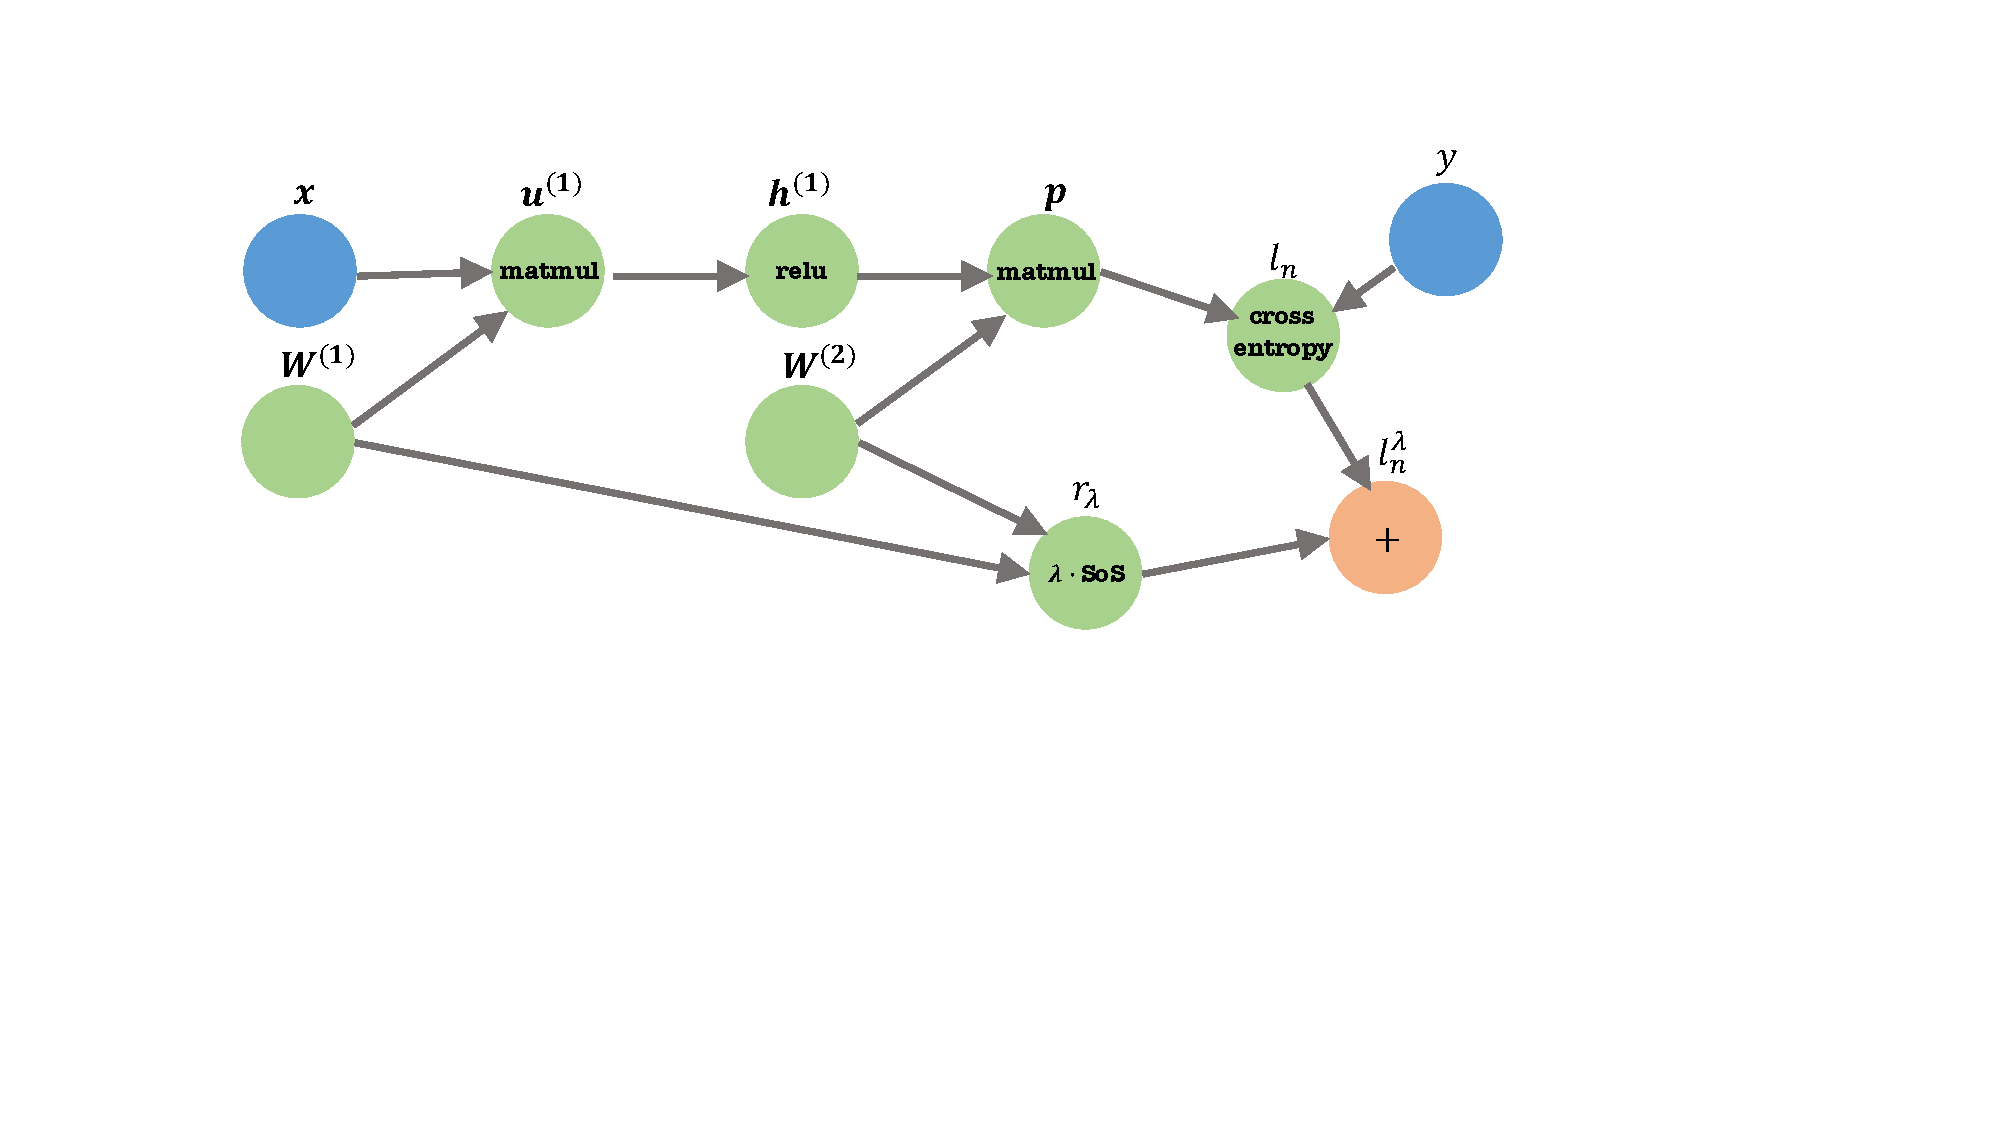
\includegraphics[width=0.75\textwidth]{compuGraph2}\caption{The computational graph illustrates the loss \eqref{eq:regloss}. For simplicity, we omit the bias terms. Symbols inside nodes represent functions, and symbols outside nodes represent function outputs (vectors/scalars). {\normalfont \texttt{matmul}} is matrix multiplication, {\normalfont \texttt{relu}} is the ReLU activation, {\normalfont \texttt{cross entropy}} is the cross entropy loss, and {\normalfont \texttt{SoS}} is the sum of squares.} \label{fig:comgraph}
\end{figure}

A more general way to think about neural network models and training is to consider \textit{computational graphs}. Computational graphs are directed acyclic graphs that represent functional relations between variables. They are very convenient and flexible to represent function composition, and moreover, they also allow an efficient way of computing gradients. Consider an MLP with a single hidden layer and an $\ell_2$ regularization:
\begin{equation}\label{eq:regloss}
\ell_{\cB}^\lambda (\btheta) = \ell_{\cB}(\btheta) + r_\lambda(\btheta) = \ell_{\cB}(\btheta) + \lambda \Big( \sum_{j,j'} \big(W_{j,j'}^{(1)}\big)^2 + \sum_{j,j'} \big(W_{j,j'}^{(2)}\big)^2 \Big),
\end{equation}
where $\ell_{\cB}(\btheta)$ is the same as \eqref{eq:loss-nn}, and $\lambda \ge 0$ is a tuning parameter. A similar example is considered in~\cite{deeplearningbook}. The corresponding computational graph is shown in Figure~\ref{fig:comgraph}. Each node represents a function (inside a circle), which is associated with an output of that function (outside a circle). For example, we view the term $\ell_{\cB}(\btheta)$ as a result of $4$ compositions: first the input data $\xx$ multiplies the weight matrix $\bW^{(1)}$ resulting in $\uu^{(1)}$, then it goes through the ReLU activation function \texttt{relu} resulting in $\hh^{(1)}$, then it multiplies another weight matrix $\bW^{(2)}$ leading to $\pp$, and finally it produces the cross-entropy with label $y$ as in \eqref{eq:crossentropy}. The regularization term is incorporated in the graph similarly.

A forward pass is complete when all nodes are evaluated starting from the input $\xx$. A backward pass then calculates the gradients of $\ell_{\cB}^\lambda$ with respect to all other nodes in the reverse direction. Due to the chain rule, the gradient calculation for a variable (say, $\partial \ell_{\cB} / \partial \uu^{(1)}$) is simple: it only depends on the gradient value of the variables ($\partial \ell_{\cB} / \partial \hh$) the current node points to, and the function derivative evaluated at the current variable value ($\bsigma'(\uu^{(1)})$). Thus, in each iteration, a computation graph only needs to (1) calculate and store the function evaluations at each node in the forward pass, and then (2) calculate all derivatives in the backward pass.

Back-propagation in computational graphs forms the foundations of popular deep learning programming softwares, including TensorFlow~\citep{tensorflow2015-whitepaper} and PyTorch~\citep{paszke2017automatic}, which allows more efficient building and training of complex neural net models.  %There are many techniques for building modules in computational graphs, which we shall see in Section~\ref{sec:pop}.

\subsection{Some general remarks}

We give a few remarks about general characteristics of deep neural network models and training. Specific deep neural network models and training are detailed in later sections.
Before we move on to introducing various popular models in deep learning, we pause here to single out several distinctive characteristics of deep neural nets that are widely believed to contribute towards the success of deep learning. Further theoretical justifications are left to Section~\ref{sec:theory}. \cm{The following three paragraphs need to be revised.}

\cm{I think overparametrization might be a major reason, and it seems relevant to Statistics.}

First, during training, stochastic gradient descent (SGD) and its variants are widely used. The subsamples of SGD are typically of size 32--512, and are drawn without replacement from a training set of size from thousands to millions. A pass of the whole training set is called an \textit{epoch}. Usually, after several or tens of epochs, the validation error levels off and training is complete. \TODO{add a figure showing the typical training/test curve} There are at least two reasons why SGD is widely used: (1) it usually speeds up computation in large machine learning tasks \citep{bottou2010large}, which has been well known; (2) it can achieve optimal statistical accuracy, and even outperforms the full-batch gradient descent (that is, $\cB = [n]$) \citep{keskar2016large}. The latter is particularly intriguing from the perspective of statistics, which stirs widespread interest in recent years. See Section~\ref{sec:stochastic-opt} for details of SGD. \TODO{discuss in Section 6.}

Second, prediction performance generally improves as neural nets become deeper (e.g., 5-30 layers). Deep neural networks are usually over-parametrized, which means that the number of parameters is much larger the sample size. The benefits of depth are at least two-fold: (1) deep neural nets form a larger function space, and thus training error is typically smaller due to better fitting; (2) with explicit or even implicit regularization, the test error is also usually smaller. With regard to the first point, an interesting phenomenon is that the effect of increasing depth is much better than of increasing width. In particular, for many problems, DNNs do not seem to suffer from the curse of dimensionality. Thus, in this respect, DNNs brings new and powerful tools for efficient data fitting. The second point is intriguing from the statistical perspective, because over-parametrization would normally run the risk of severe overfitting in other models. Section~\ref{sec:approx} and~\ref{sec:generalization} provide recent theories for the the effects of depth and over-parametrization.

It is easy to understand that a larger model has more capacity for data fitting, so (1) should be well expected.  For deep nets, the benefit in data fitting, namely (1), is much more significant compared with wide shallow nets \TODO{def!}. Many traditional statistical methods such as basis expansion is analogous to shallow nets \TODO{need to discuss this before}. Thus, in this respect, deep neural nets brings very new and powerful tools for efficient data fitting. The benefit in generalization, namely (2), is exciting from the statistics standpoint. While explicit regularization through $\ell_2$ or $\ell_1$ has been well studied, implicit regularization such as SGD is recognized only recently \TODO{check; refs}.

\cm{My friend Chenxi's comment: I wouldn't agree with the second point of "several distinctive characteristics", that the deeper the better. In fact, the current best ImageNet models (e.g. mine https://arxiv.org/abs/1712.00559; better than ResNet ~5\% top-1) only has maximum depth of less than 30. "The deeper the better" may only be true in networks that rely heavily on residual connections.}

Third, the ReLU activation function is a crucial element in most deep learning architectures. \TODO{add a figure to show different activation functions} Its popularity is largely due to the fact that its derivative is either $0$ or $1$, which makes training more efficient. Note that in back-propagation, gradient calculation is multiplicative due to the recursive relation \eqref{eq:grad}. Thus, it is important to keep gradients from being ``killed'', which means that gradients become approximately zero if in the multiplication a factor $\sigma'$ is very small due to an input with large magnitude. Historically, the sigmoid function (a.k.a.\ the logistic function) was the common choice for the activation function, but for deep neural nets, it tends to kill gradients and has inferior training performance \citep{krizhevsky2012imagenet, maas2013rectifier}. In contrast, ReLU or its variants (e.g., leaky ReLU) is much better for training as well as parameter initialization.

\subsection{Numerical experiments}

\begin{lstlisting}[language=Python]
from keras.datasets import mnist
from keras.models import Sequential
from keras.layers import Dense, Flatten

# the data, split between train and test sets
(x_train, y_train),(x_test, y_test) = mnist.load_data()
x_train, x_test = x_train / 255.0, x_test / 255.0

MLP = Sequential([
 Flatten(),
 Dense(512, activation=tf.nn.relu),
 Dense(10, activation=tf.nn.softmax)
])
MLP.compile(optimizer='sgd',
             loss='sparse_categorical_crossentropy',
             metrics=['accuracy'])

MLP.fit(x_train, y_train, epochs=5, batch_size=32,
         verbose=1,
         validation_split=0.1)
score = MLP.evaluate(x_test, y_test)
\end{lstlisting}

%%%%%%%%% Below are some good links
% How PyTorch implements autograd: https://towardsdatascience.com/getting-started-with-pytorch-part-1-understanding-how-automatic-differentiation-works-5008282073ec
% On activation functions: https://medium.com/@kanchansarkar/relu-not-a-differentiable-function-why-used-in-gradient-based-optimization-7fef3a4cecec

